% ------------------------------------------------------------------------------
%
% PREAMBLE
%
% ------------------------------------------------------------------------------

\documentclass[12pt, titlepage]{article}


\usepackage{graphicx, amsmath, amssymb, natbib, setspace, sectsty, verbatim, 
		mathrsfs, float}
\usepackage{MnSymbol}
\usepackage{multirow}
\usepackage{bm}
\usepackage[usenames, dvipsnames]{color}
\bibpunct{(}{)}{;}{a}{}{,}
\setlength{\parindent}{3em}
%\parskip = 1.5ex
%\linespread{1.3}
%\onehalfspacing

\pdfpagewidth 8.5in
\pdfpageheight 11in
\setlength{\oddsidemargin}{0.0in} \setlength{\textwidth}{6.5in}
\setlength{\topmargin}{0.15in} \setlength{\textheight}{8.5in}
\setlength{\headheight}{0.0in} \setlength{\headsep}{0.0in}

\usepackage{/mnt/ExtraDrive1/Work/shTex/mymacros}

\providecommand{\norm}[1]{\lVert#1\rVert}
\newcommand{\csection}[1]{\section[#1]{\centering #1 }}
\subsectionfont{\small}
\newcommand{\cye}[1]{\color{yellow!70!black}#1}
\newcommand{\cre}[1]{\color{red!70!black}#1}
\newcommand{\cbl}[1]{\color{blue!70!black}#1}
\newcommand{\cgr}[1]{\color{green!70!black}#1}


% ------------------------------------------------------------------------------
%
% BEGIN DOCUMENT
%
% ------------------------------------------------------------------------------

\begin{document}

\setcounter{equation}{0}
\renewcommand{\theequation}{R.\arabic{equation}}


% ------------------------------------------------------------------------------
%
%                    Section 8.8.1
%                    Seal trend data
%
% ------------------------------------------------------------------------------

{\large \flushleft \textbf{8.8.1 Seal trend data}}

\vspace{.3cm}

Models for the harbor seal data are based on neighborhood relationships (Figure 1.3) which leads to linear models based on spatial weights (Chapter 7). In general, these types of models are amenable to fast computing because they are specified through the inverse of the covariance matrix, e.g., $\boldsymbol{\Sigma}^{-1} = \mathbf{K}_{\textrm{CAR}}(\mathbf{I} - \rho_{\textrm{CAR}}\mathbf{W})$ (eq. 7.7 using the parsimonious models in Section 7.2).  It is the inverse of the covariance matrix that is used in the likelihoods (e.g, eqns 8.1 and 8.2), and this can be computationally demanding for large data sets if the models are specified through the covariance matrix, such as the geostatistical models (Chapter 6).  Both geostatistical and spatial-weights models also require $|\boldsymbol{\Sigma}^{-1}|$ in the likelihood, and there are special algorithms for sparse matrices such as those for the spatial-weights models.  Hence, the spatial-weights models would seem to have a computational advantage over the geostatistical models.

However, one interesting aspect of the harbor seal example is that it contains missing data.  Ultimately, we will want to predict at these missing locations, so, for the spatial-weights models, we must include the missing locations in the neighborhood structure.  Recall that for the likelhood evaluations and optimization, we need the inverse of the covariance matrix for \textit{only} the observed data, resulting in a situation where the computational advantages of the spatial-weights models can vanish. To make this clear, let us order the locations so that all of the observed locations are first, followed by the unobserved locations, and then the covariance matrix and inverse of the covariance matrix are
$$
    \boldsymbol{\Sigma} = 
    \begin{bmatrix}
       \boldsymbol{\Sigma}_{oo} & \boldsymbol{\Sigma}_{ou} \\
       \boldsymbol{\Sigma}_{uo} & \boldsymbol{\Sigma}_{uu}
    \end{bmatrix}  \ \textrm{ and } \  
    \bSigma^{-1} = 
    \begin{bmatrix}
       \boldsymbol{\Sigma}^{oo} & \boldsymbol{\Sigma}^{ou} \\
       \boldsymbol{\Sigma}^{uo} & \boldsymbol{\Sigma}^{uu}
    \end{bmatrix}, 
$$
where the subscripts and superscripts $o$ and $u$ are for the observed and unobserved locations, respectively. The most straight-forward idea for the spatial-weights models is to obtain the covariance matrix $\boldsymbol{\Sigma}_{oo}$ by first taking $\boldsymbol{\Sigma} = (\boldsymbol{\Sigma}^{-1})^{-1}$, and then computing $\boldsymbol{\Sigma}_{oo}^{-1}$ because, unfortunately, $\boldsymbol{\Sigma}_{oo}^{-1} \neq \boldsymbol{\Sigma}^{oo}$, and, also $\boldsymbol{\Sigma}_{oo}^{-1} \neq (\boldsymbol{\Sigma}^{oo})^{-1}$. However, there is a faster way than taking the two inverses $(\boldsymbol{\Sigma}^{-1})^{-1}$ and $\boldsymbol{\Sigma}_{oo}^{-1}$, by recalling from Section 5.6 that if we already have $\boldsymbol{\Sigma}^{-1}$, then we can obtain 
$$
    \boldsymbol{\Sigma}_{oo}^{-1} = \boldsymbol{\Sigma}^{oo} - \boldsymbol{\Sigma}^{ou} (\boldsymbol{\Sigma}^{uu})^{-1} \boldsymbol{\Sigma}^{uo},
$$
which requires a single numeric inverse $(\boldsymbol{\Sigma}^{uu})^{-1}$ that has dimensions less than those of the full $(\boldsymbol{\Sigma}^{-1})^{-1}$, and will be very beneficial of the dimensions of $\boldsymbol{\Sigma}_{uu}$ are (much) less than $\boldsymbol{\Sigma}_{oo}$.  If the dimensions of $\boldsymbol{\Sigma}_{uu}$ are (much) larger than $\boldsymbol{\Sigma}_{oo}$, then the spatial-weights models, in terms of the computational demand due to matrix inverses, are more costly than geostatistical models.  For the harbor seal example, there were 306 observed locations and 157 missing locations, so we only needed a $157 \times 157$ inverse. 

We want to fit models by maximizing the log-likelihood for a variety of spatial-weights models. Figure 1.3 shows first, second, and fourth-order neighborhood relationships.  If $\mathbf{W}_{1}$ is a symmetric spatial-weights matrix as described in Chapter 7, then a matrix that includes ``neighbors of neighbors'' is
$$
\mathbf{W}_{2} = \mathcal{I}(\mathcal{I}(\mathbf{W}_{1}\mathbf{W}_{1} > 0) + \mathbf{W}_{1} > 0) - \mathbf{I}
$$
where $\mathcal{I}(\cdot)$ is the indicator function, equal to 1 if its argument is true, otherwise it is zero, and $\mathbf{I}$ is the identity matrix to ensure that the diagonal of $\mathbf{W}_{2}$ is all zeros.  In a similar fashion, we can create a fourth-order neighborhood matrix, $\mathbf{W}_{4}$ from $\mathbf{W}_{2}$.  Also, recall that for these data we have a single explanatory variable, which is a categorical (factor) variable for one of five different genetic stocks (Figure 1.1).

\begin{figure}[H]
  \begin{center}
	    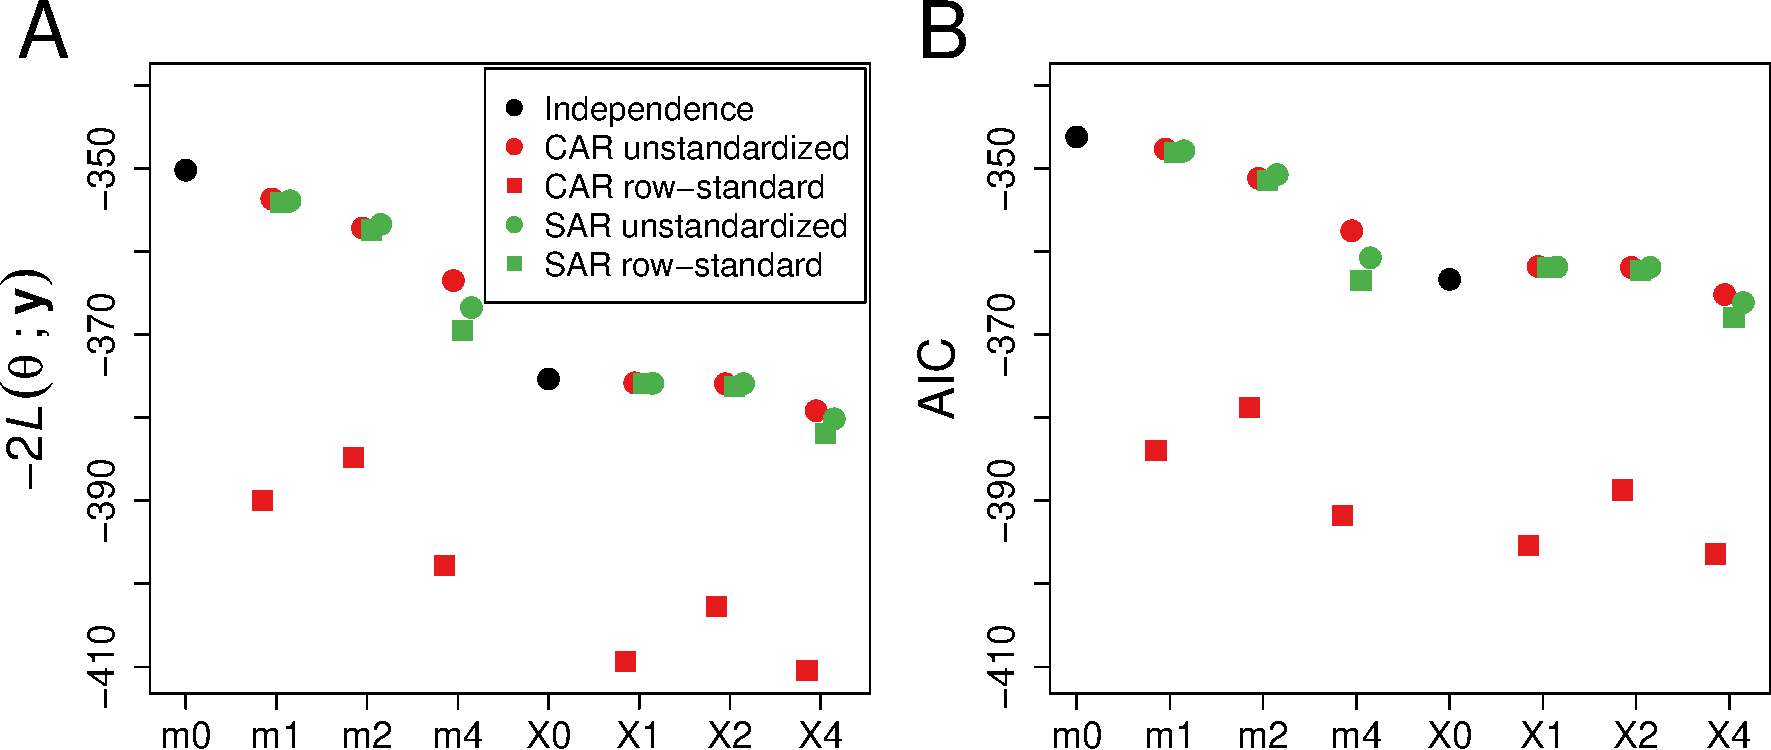
\includegraphics[width=1\linewidth]{Seals_m2LL_AIC}
  \end{center}
  \caption{Log-likelihood and AIC.  \label{Fig:Seals_m2LLAIC}}
\end{figure}

For the harbor seal example, we want to consider a variety of models that include whether or not a spatially-autocorrelated error structure is even necessary, and if so, whether it should be a CAR or SAR model.  In both cases, we also can consider the first, second, and fourth-order neighborhood models as described above, and whether or not row-standardization was applied to those binary matrices. Figure~\ref{Fig:Seals_m2LLAIC} shows $-2L(\boldsymbol{\theta};\mathbf{y})$ (eq. 8.1) and AIC for all of these models.  Generally, we see that models including the explanatory variable fit better than those without it.  Interestingly, for the models with stock as an explanatory variable, the fit for CAR and SAR unstandardized, and SAR standardized, for first and second order neighbors is almost identical to the independence model, and so there AIC favors the independence model because the spatial models have one more parameter (here, the spatial covariance can be thought of as $\boldsymbol{\Sigma} = \sigma^{2}\mathbf{R}_{\rho}$, where $\sigma^{2}$ is an overall variance parameter and $\mathbf{R}_{\rho}$ is a CAR or SAR covariance matrix that depends on the single parameter $\rho$.  The most dramatic feature of Figure~\ref{Fig:Seals_m2LLAIC} is the much improved fit when using row-standardization with the CAR models.  The best overall models suggested by AIC were the first and fourth-order, row-standardized CAR models that had stock as an explanatory variable.

Because there are only 2 covariance parameters, it is very instructive to look at the restricted log-likelihood for the variance and range parameters.  Consider the model
\begin{equation} \label{eq:seals_splm}
\mathbf(y) = \mathbf{X}\boldsymbol{\beta} + \boldsymbol{\varepsilon},
\end{equation}
where $\mathbf{X}$ contains indicator variables for genetic stock membership, and $\boldsymbol{\varepsilon}$ has a CAR covariance matrix
$$
\var(\boldsymbol{\varepsilon}) = \sigma^{2}(\mathbf{D} - \rho\mathbf{W}_{4})^{-1}
$$
where $\mathbf{D}$ is a diagonal matrix with elements $\mathbf{W}_{4}\mathbf{1}$, $\mathbf{1}$ is a vector of all ones, and recall that $\mathbf{W}_{4}$ is the fourth-order neighborhood matrix. Note that this is an equivalent way to write a CAR model with row-standardization (Section 7.3). The resulting log-likelihood surface is shown in Figure~\ref{Fig:Seals_logLik}, and the restricted maximum likelihood estimate is the value at the maximum of this surface, shown as a black circle, where $\hat{\rho} = 0.761$ and $\hat{\sigma}^{2} = 0.267$.  There are several ways to make inference on the covariance parameters, including profile likelihood and Fisher's Information matrix.
\begin{figure}[H]
  \begin{center}
	    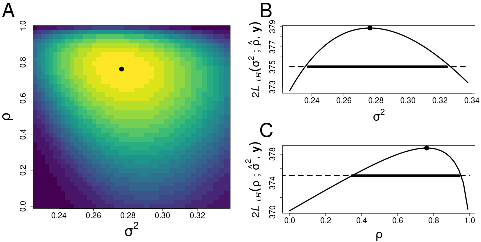
\includegraphics[width=1\linewidth]{Seals_logLik}
  \end{center}
  \caption{Restricted log-likelihood surface.  \label{Fig:Seals_logLik}}
\end{figure}

Consider the REML log-likelihood function in Section 8.2, which here is denoted as $L_{-i,R}(\theta_{i};\hat{\boldsymbol{\theta}}_{-i},\mathbf{y})$, where the $i$th component of $\boldsymbol{\theta}$ has been held constant at $\theta_{i}$, and the function has been maximized for all other parameters, whose values are denoted as $\hat{\boldsymbol{\theta}}_{-i}$.  For our model, $\boldsymbol{\theta} = (\rho, \sigma^{2})$.  Note that $\hat{\boldsymbol{\theta}}_{-i}$ changes with each $i$, but we suppress any notation to indicate such dependence. Then a profile likelihood plot for the $i$th component of $\boldsymbol{\theta}$ is one that plots $2L_{-i,R}(\theta_{i};\hat{\boldsymbol{\theta}}_{-i},\hat{\boldsymbol{\beta}},\mathbf{y})$ for various values of $\theta_{i}$, and these are seen in Figure~\ref{Fig:Seals_logLik}B for $\sigma^{2}$ and Figure~\ref{Fig:Seals_logLik}C for $\rho$.  A $1-\alpha$ level confidence interval for $\theta_{i}$ can be obtained by finding all values of $\theta_{i}$ in the profile likelihood where $2L_{-i,R}(\theta_{i};\hat{\boldsymbol{\theta}}_{-i},\mathbf{y})$ are greater than $\hat{\theta}_{i} - \chi^{2}(1-\alpha,1)$, where $\chi^{2}(x;\nu)$ is a quantile function, $0 \le x \le1$, of a chi-squared distribution on $\nu$ degrees of freedom. Using $\alpha = 0.05$ leads to a 95\% confidence interval and the well-known value of $\chi^{2}(0.95,1) = 3.841$, and $\hat{\theta}_{i} - 3.841$ are shown by the dashed lines in Figure~\ref{Fig:Seals_logLik}B,C. The confidence interval is the solid horizontal line, above which all values of $L_{-i,R}(\theta_{i};\hat{\boldsymbol{\theta}}_{-i},\hat{\boldsymbol{\beta}},\mathbf{y})$ are greater than $\hat{\theta}_{i} - 3.841$. For $\rho$, the 95\% confidence interval is from 0.347 to 0.941, and for $\sigma^{2}$, it is from 0.238 to 0.324. 

A second approach to finding a confidence interval is based on large sample asymptotics, where the curvature of the likelihood in Figure~\ref{Fig:Seals_logLik} at the REMLE (or we could also use MLE) is approximated by the observed Fisher's Information matrix, which can be used to construct confidence intervals as suggested in Section 8.4.  After fitting the model, we compute 
$$
\boldsymbol{J}_{a}{(\boldsymbol{\theta})_{i,j}} = \frac{1}{2}\operatorname{tr}\left(\boldsymbol{\Sigma}^{-1} \frac{\partial \boldsymbol{\Sigma}}{\partial\theta_i}{\boldsymbol{\Sigma}^{-1}}\frac{\partial\boldsymbol{\Sigma}}{\partial\theta_j}\right),
$$
by using $\boldsymbol{\Sigma}^{-1} = (\mathbf{D} - \hat{\rho}\mathbf{W})/\hat{\sigma}^{2}$ and noting that 

\begin{align*}
	\frac{\partial \boldsymbol{\Sigma}}{\partial\sigma^{2}} = & (\mathbf{D} - \rho\mathbf{W}_{4})^{-1}, \\
	\frac{\partial \boldsymbol{\Sigma}}{\partial\rho} = & \sigma^{2}(\mathbf{D} - \rho\mathbf{W}_{4})^{-1}\mathbf{W}_{4}(\mathbf{D} - \rho\mathbf{W}_{4})^{-1},
\end{align*}
where $\sigma^{2}$ and $\rho$ are replaced by $\hat{\sigma}^{2}$ and $\hat{\rho}$, respectively. 

An estimator of the asymptotic standard errors of $\hat{\boldsymbol{\theta}}$ are the square roots of the diagonal of $[\boldsymbol{J}_{a}{(\boldsymbol{\theta})}]^{-1}$.  Formally, let $\mathbf{j}_{i}$ be a vector of all zeros, except there a single one at the $i$th element.  Then a $(1 - \alpha)100$\% confidence interval for $\hat{\theta}_{i}$ is
$$
\hat{\theta}_{i} \pm z_{1-\alpha/2}\sqrt{\mathbf{j}_{i}^{T}[\boldsymbol{J}_{a}{(\boldsymbol{\theta})}]^{-1}\mathbf{j}_{i}},
$$
where $z_{1-\alpha/2}$ is a quantile of a standard normal distribution at $1-\alpha/2$.  For example, if $\alpha = 0.05$, then $z_{1-\alpha/2}$ is the familiar 1.96.  In our example, the standard errors for $\rho$ and $\sigma^{2}$ were 0.101 and 0.018, respectively, so the 95\% confidence interval for $\rho$ was from 0.563 to 0.959 and for $\sigma^{2}$ it was from 0.240 to 0.312, which can be compared to those obtained from profile likelihood.

Another approach is to compute the Hessian matrix of the log-likelihood.  We used \texttt{spmodel} for this as it allowed us to evaluate the log-likelihood for any given value of $\boldsymbol{\theta}$.  We used the \texttt{R} package \texttt{numDeriv} to compute the numeric Hessian, $\mathbf{H}$, at the REMLE, and then an estimator of Fisher's Information is,
$$
\boldsymbol{J}_{n}{(\boldsymbol{\theta})} = -\mathbf{H},
$$
and an estimator of the asymptotic standard errors follow in exactly the same way as they were developed when using $\boldsymbol{J}_{a}{(\boldsymbol{\theta})}$.  In our example, the standard errors for $\rho$ and $\sigma^{2}$ were 0.145 and 0.023, respectively, so the 95\% confidence interval for $\rho$ was from 0.476 to 1.046 and for $\sigma^{2}$ it was from 0.231 to 0.321, which can be compared to those obtained from the analytical computation of Fisher's Information and profile likelihood.  Here, the confidence interval for $\rho$ extends beyond 1 at the upper bound, showing a disadvantage of the large-sample asymptotic approach that relies on normality.

Nevertheless, it is interesting to look at the asymptotic correlation among the parameters as revealed by the observed Fisher's Information matrix.  Let $\mathbf{S}_{a}$ be a diagonal matrix containing reciprocals of the square roots from the diagonal of $[\boldsymbol{J}_{a}{(\boldsymbol{\theta})}]^{-1}$, and similarly obtain $\mathbf{S}_{n}$ from $[\boldsymbol{J}_{n}{(\boldsymbol{\theta})}]^{-1}$ .  Then estimators of the asymptotic correlation matrix are
$$
\mathbf{S}_{a}[\boldsymbol{J}_{a}{(\boldsymbol{\theta})}]^{-1}\mathbf{S}_{a} =
\left(
\begin{array}{rr}
1.000 & 0.163 \\ 
  0.163 & 1.000  \\ 
\end{array}
\right) \textrm{ and }
\mathbf{S}_{n}[\boldsymbol{J}_{n}{(\boldsymbol{\theta})}]^{-1}\mathbf{S}_{n} =
\left(
\begin{array}{rr}
1.000 & -0.189 \\ 
  -0.189 & 1.000  \\ 
\end{array}
\right),
$$
which show little correlation between $\rho$ and $\sigma^{2}$, and this is also evident in the shape of the log-likelihood surface (Figure~\ref{Fig:Seals_logLik}A).
 
One of the features of the spatial-weights models is that they are nonstationary, and it is interesting to investigate this property for actual data.  First, consider two models as in \eqref{eq:seals_splm}, using the fourth-order neighborhood structure, one where the $\mathbf{W}$ is standardized, i.e., $\var(\boldsymbol{\varepsilon}) = \boldsymbol{\Sigma}_{rs} = \sigma^{2}_{rs}(\mathbf{I} - \rho_{rs}\overline{\mathbf{W}}_{4})\mathbf{K}_{rs}$, and the other where it is not, i.e., i.e., $\var(\boldsymbol{\varepsilon}) = \boldsymbol{\Sigma}_{un} = \sigma^{2}_{un}(\mathbf{I} - \rho_{un}\mathbf{W}_{4})\mathbf{K}_{un}$. The diagonal elements of $\boldsymbol{\Sigma}_{rs}$, plotted as a function of the number of neighbors, is shown in Figure~\ref{Fig:seals_nonstationary}A.
 \begin{figure}[H]
  \begin{center}
	    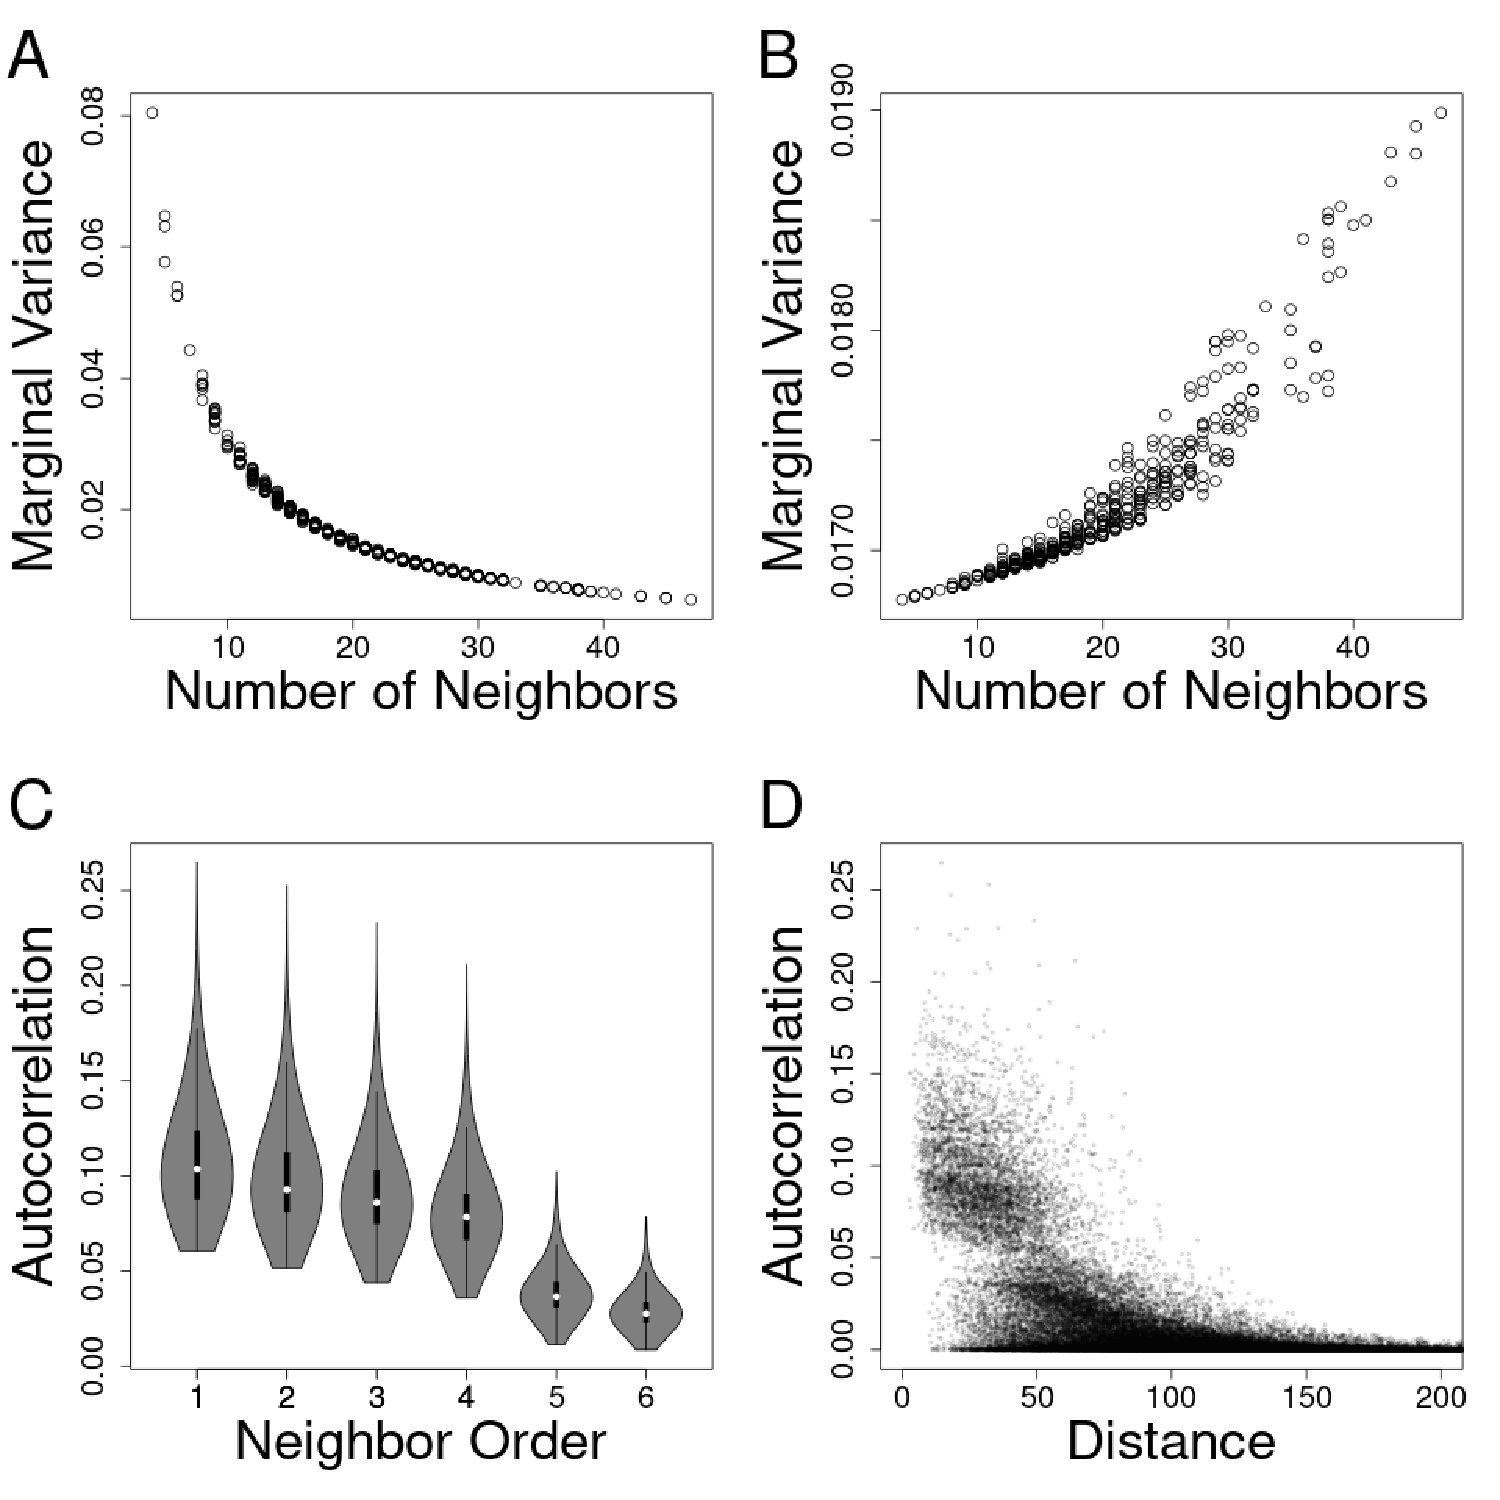
\includegraphics[width=.8\linewidth]{Seals_nonstationary}
  \end{center}
  \caption{adfafd. \label{Fig:seals_nonstationary}}
\end{figure}


Let us consider the Matern covariance function, which is very popular because it has an additional parameter that controls smoothness and differentiability of the surface that it produces.  In Table 6.1, this is denoted at $\theta_{3}$, and we will call it the smoothness parameter. If $\theta_{3} = 1/2$, then the Matern model is equivalent to the exponential model, if $\theta_{3} = 1$ is has been called the Whittle model, if $\theta_{3} = 3/2$ it is a radon model of order 2, if $\theta_{3} = 5/2$ it is a radon model of order 4, and as $\theta_{3} \rightarrow \infty$, the Matern model is equivalent to a Gaussian model.  In \texttt{spmodel}, the smoothness parameter is allowed to range from $1/5$ to 5.  For the Matern model, Figure~\ref{Fig:Matern_SO4}  shows the profile likelihood decreasing slowly as values for the partial sill and range increase beyond their REMLEs.  The nugget has a pronounced peak in the profile likelihood.  Some authors claim that the smoothness parameter for the Matern model is difficult to estimate, and they suggest either picking a single value, or pick several, and choose one based on the likelihood or other model selection criteria.  However, for these data, the smoothness parameter has a fairly well-defined maximum, and optimization had no issues.

\vspace{.3cm}

{\large \flushleft \textbf{9.10.2 Prediction of wet sulfate deposition}}

\vspace{.3cm}

We continue with our analysis from Section 8.8.3 of the clean wet sulfate deposition data in the conterminous U.S.  Our ultimate goal will be to create a map, with prediction intervals, on a grid of prediction locations across the whole U.S. that will help us assess the spatial patterns in wet sulfate deposition along with our confidence in those predictions.  We left some model selection choices open from Section 8.8.3 because predictive ability of those models will help in our selection process.  We will complete the analysis here, and begin with leave-one-out cross-validation (LOOCV).

LOOCV eliminates one datum at a time, using all of the rest of the data to predict the one that was removed.  There is a fast and a slow way to do this.  The slow way is to remove a datum and then re-estimate all of the parameters using ML or REML estimation each time.  However, with the removal of but a single datum, the parameter estimates change very little.  A fast way to achieve LOOCV is based on holding all parameters at their values as estimated by using all of the data, and then using results from partitioned matrices so that we only have to invert the covariance matrix once (which can be saved from the ML or REML estimation, so there is in fact no additional matrix inverses are required).  Recall from Section 5.6 that,
if a matrix is partitioned as,
$$
    \boldsymbol{\Sigma} = 
    \begin{bmatrix}
       \boldsymbol{\Sigma}_{11} & \boldsymbol{\Sigma}_{12} \\
       \boldsymbol{\Sigma}_{21} & \boldsymbol{\Sigma}_{22}
    \end{bmatrix}  \ \textrm{ and } \  
    \bSigma^{-1} = 
    \begin{bmatrix}
       \boldsymbol{\Sigma}^{11} & \boldsymbol{\Sigma}^{12} \\
       \boldsymbol{\Sigma}^{21} & \boldsymbol{\Sigma}^{22}
    \end{bmatrix}, 
$$
then 
$$
    \boldsymbol{\Sigma}_{11}^{-1} = \boldsymbol{\Sigma}^{11} - \boldsymbol{\Sigma}^{12} (\boldsymbol{\Sigma}^{22})^{-1} \boldsymbol{\Sigma}^{21}.
$$
Moreover, let us order the data such that the datum to be removed is last, so that $\boldsymbol{\Sigma}^{22}$ is a scalar, then the inverse of $\boldsymbol{\Sigma}^{22}$ is trivial and $\bSigma_{11} \upi$ can be computed rapidly. The main computational expense of kriging predictions rely on the inverse covariance matrix for the observed data, but in LOOCV that is given by $\bSigma_{11} \upi$, which is computed rapidly without any further matrix inverses if we already have $\bSigma \upi$. The only other quantity from $\boldsymbol{\Sigma}$ needed for prediction is the vector $\boldsymbol{\Sigma}_{12}$.  Conceptually, we just re-order the data, one at a time, putting the one to be removed last in the covariance matrices above, and that allows the predictions to be computed quickly.

Let $\hat{y}_{i} = \bar{u}$ from (9.2) be the $i$th predicted value using LOOCV where the $i$th datum has been removed, and let $\hat{v}_{i} = \sqrt{\var(\bar{u} - u)}$ from (9.3) be the $i$ prediction standard error.  Then we will consider two metrics to assess model performance.  One is the root-mean-squared prediction error (RMSPE), which we computed as
$$
\sqrt{\frac{1}{n}\sum_{i=1}^{n} (\hat{y}_{i} - y_{i})^{2} }.
$$
Models with lower RMSPE have better predictive performance.  The other metric is the 90\% prediction interval coverage, PIC90, which we computed as
$$
\frac{1}{n} \sum_{i=1}^{n} \mathcal{I}(\hat{y}_{i} - z_{1-\alpha/2}v_{i} \le y_{i} \le \hat{y}_{i} + z_{1-\alpha/2}v_{i}),
$$
where $\mathcal{I}(\cdot)$ is an indicator function, equal to 1 if its argument is true, and 0 otherwise, and $z_{1-\alpha/2}$ is a standard normal value below which contains $1-\alpha/2$ of the probability density.  We chose $\alpha = 0.1$ for PIC90, resulting in the familiar $z_{0.95} = 1.645$.

One problem with LOOCV is that it may be overly optimistic in assessing actual prediction.  A simple thought experiment reveals why.  Suppose 99 data locations were clustered very closely together, and another was separated from the cluster.  Then, for LOOCV, as we removed each datum from the cluster, we would have many nearby locations and get very precise predictions with small prediction standard errors, and they would swamp RMSPE and PIC90 if our overall goal was to predict in a region that was substantially larger than that enclosing the cluster of locations. The same is essentially true if all locations were pairs of locations that were very close to each other, but the pairs were scattered.  Still, under normal sampling scenarios, it can be a good way to evaluate models as they are all operating under the same sampling scheme.

A second way to use cross-validation is called $n$-fold cross-validation.  Here we divide the data into $n$ groups, and remove one whole group to be predicted -- this is often called the \textit{test} dataset.  The remaining data are called the \textit{training} dataset, and are used to fit a model and make predictions at the locations of the test dataset.  Then, the predictions at the locations for the test dataset can be compared to the actual values that were removed.  In fact, RMSPE and PIC90 can be computed for $n$-fold cross-validation in exactly the same way as for LOOCV, and to distinguish them, we use RMSPE$_{\textrm{Lo}}$ and PIC90$_{\textrm{Lo}}$ for LOOCV, and RMSPE$_{\textrm{Nf}}$ and PIC90$_{\textrm{Nf}}$ for $n$-fold cross-validation. With $n$-fold cross-validation we do not have to fit the model as many times, so we completely re-fit the model for each group that is removed.  Groups are often created randomly, and we will do it this way too.  If we want to get the best feel how well a model will interpolate, that includes even a bit of extrapolation at the edges, it is desirable to have just a few groups.  This may be more pessimistic about model performance than the real data because we are decreasing our sample sizes substantially.  Nevertheless, to examine both extremes, where LOOCV is overly optimistic, we used 3-fold cross-validation, which is overly pessimistic.  Because we created 3 groups randomly, we would like to ensure that our results do not depend too much on any particular randomized grouping.  Hence, we do 3-fold cross-validation 10 times, and average the results for RMSPE (by first averaging the mean-squared prediction error, and then taking the square root) and PIC90.

To further evaluate the models from from Section 8.8.3, we will consider LOOCV and 3-fold crossvalidation for polynomials with orders up to 5, again using the exponential autocovariance model.  RMSPE using LOOCV for the independence models generally goes down with increasing order of the polynomial surface (Figure~\ref{Fig:SO4_crossval}A), suggesting, like AIC and BIC, that among this set of models, a 4th or 5th order polynomial is best.  However, when it comes to predictive performance, the spatial models are much superior, having average deviations from true values of around 0.47 for lower order polynomials, versus approximately 0.53 for the higher order polynomials of the independence models, which translates to prediction intervals that are over 11\% shorter.  The problem of over-fitting polynomials is revealed more clearly by 3-fold cross-validation (Figure~\ref{Fig:SO4_crossval}C), where the RMSPE begins to increase rapidly for the independence models for the 5th order polynomial, and increases throughout for the spatial models. It also appears that for the spatial models in both Figure~\ref{Fig:SO4_crossval}A,C that REMLE is just slightly better than MLE.

\begin{figure}[H]
  \begin{center}
	    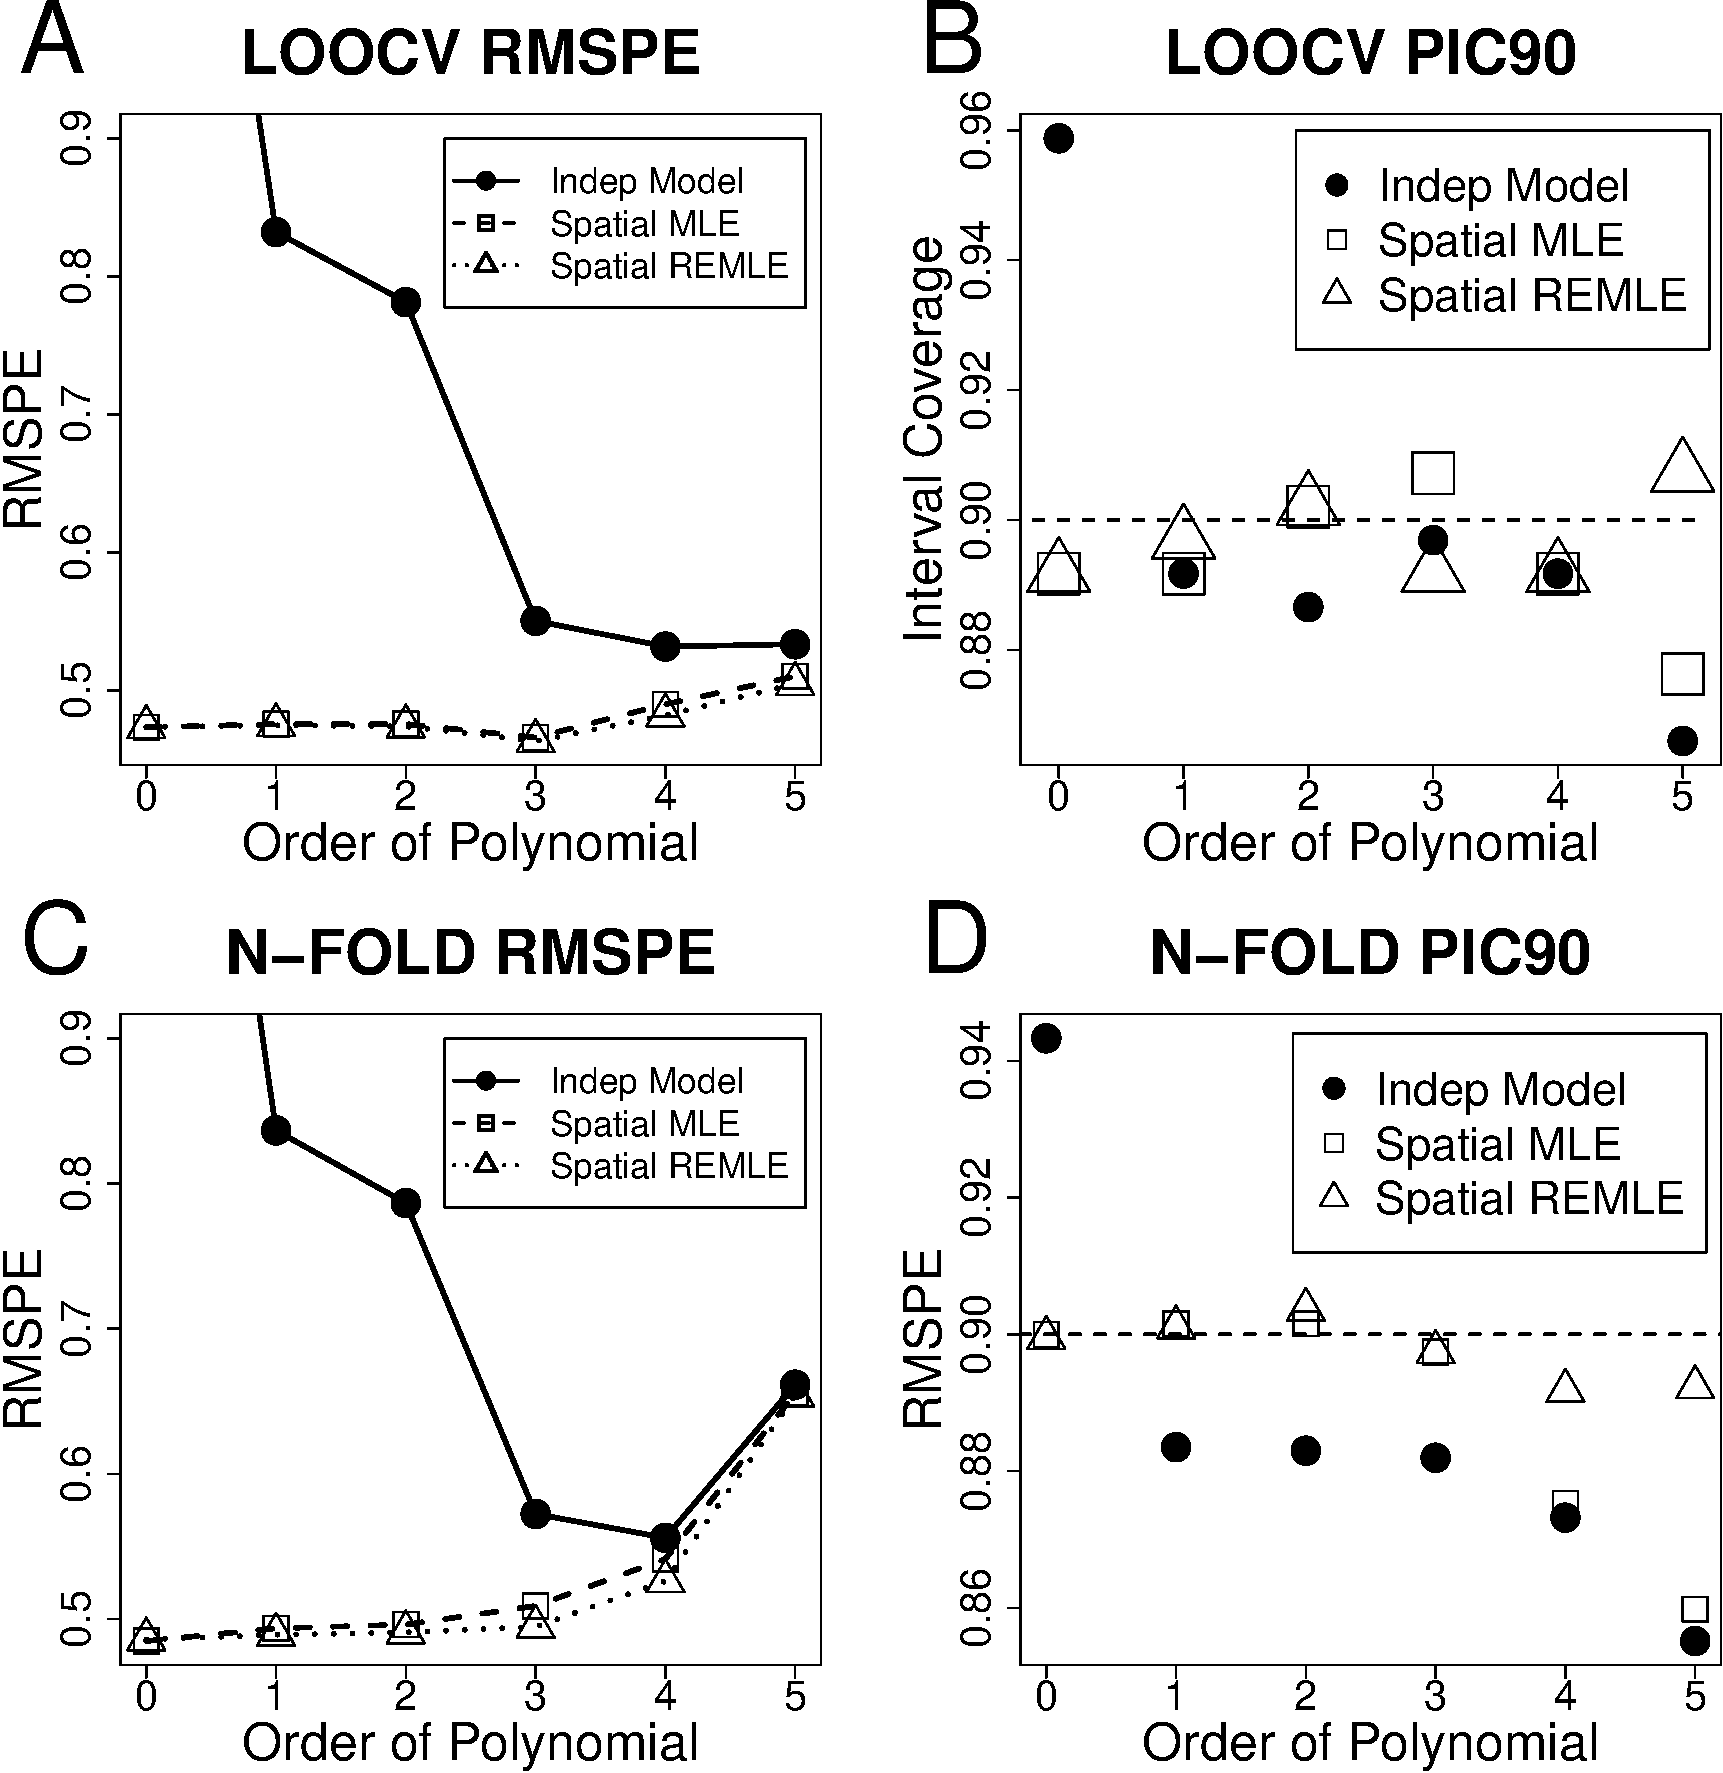
\includegraphics[width=.8\linewidth]{SO4_crossval}
  \end{center}
  \caption{Root-mean-squared prediction error (RMSPE) and 90\% prediction intervals coveraga (PIC90) using leave-one-out cross-validation (LOOCV) and 3-fold cross-validation for up to 5th order polynomial surfaces using the clean wet sulfate deposition data.  The spatial models were fit with an exponential autocovariate model using both MLE and REMLE. A. LOOCV RMSPE B. LOOCV PIC90 C. 3-fold RMSPE, and D. 3-fold PIC90. \label{Fig:SO4_crossval}}
\end{figure}

We want our prediction surfaces to be as precise as possible, but we also need to evaluate whether the estimated prediction standard-errors are valid.  By valid, we mean that a 90\% prediction interval should contain the true value 90\% of the time. For the independence models, that is approximately true for polynomial surfaces with orders 1 through 4, but the constant mean model is overly conservative (intervals that are larger than needed and thus containing the true values almost 96\% of the time, Figure~\ref{Fig:SO4_crossval}B, and 94\%, Figure~\ref{Fig:SO4_crossval}D), while the 5th order polynomial is overly optimistic (intervals that are too short and only contain the true value around 86\% of the time (Figure~\ref{Fig:SO4_crossval}B,D). The REML estimates are very close to the nominal value for all orders of the polynomial surface, while the ML estimates start to become too optimistic at order 4 using 3-fold cross-validation (Figure~\ref{Fig:SO4_crossval}D) and order 5 using LOOCV (Figure~\ref{Fig:SO4_crossval}B).

For the spatial models, based on BIC, LOOCV, and 3-fold cross-validation, there appears to be little reason to go beyond ordinary kriging.  However, we still need to choose an autocovariance model.  We fit most of the models in Table 6.1 using \texttt{spmodel}, and computed all of the model selection metrics discussed so far (Table~\ref{tab:ModelSelAutocov}).  With the exception of a few models like wave and J-Bessel, all models performed similarly. Also note that with a constant mean model, there was very little difference between LOOCV and 3-fold cross-validation. The spherical model is just slightly better than most others based on AIC, BIC, and RMSPE.  It also appears to have appropriate prediction interval coverage, so we will choose the spherical model for further analyses.
\begin{table}[h] 
				\caption{Performance metrics for various covariance functions used with a constant mean model fit with REMLE for the clean wet sulfate data. \label{tab:ModelSelAutocov}}
\begin{center}
\begin{tabular}{c|rrrrrrr}
  \hline
  \hline
  Model & m2LL & AIC & BIC & RMSPE$_{\textrm{Lo}}$ & RMSPE$_{\textrm{Nf}}$ & PIC90$_{\textrm{Lo}}$ & PIC90$_{\textrm{Nf}}$ \\
	\hline
  \hline
exponential & 302.4 & 308.4 & 318.2 & 0.473 & 0.473 & 0.892 & 0.907 \\ 
  spherical & 298.8 & 304.8 & 314.6 & 0.469 & 0.470 & 0.887 & 0.902 \\ 
  gaussian & 308.5 & 314.5 & 324.3 & 0.487 & 0.490 & 0.871 & 0.907 \\ 
  circular & 302.6 & 308.6 & 318.4 & 0.474 & 0.480 & 0.892 & 0.897 \\ 
  pentaspherical & 299.5 & 305.5 & 315.3 & 0.470 & 0.470 & 0.887 & 0.902 \\ 
  wave & 323.4 & 329.4 & 339.2 & 0.510 & 0.515 & 0.902 & 0.892 \\ 
  jbessel & 328.9 & 334.9 & 344.7 & 0.530 & 0.527 & 0.902 & 0.892 \\ 
  gravity & 301.2 & 307.2 & 317.0 & 0.477 & 0.479 & 0.887 & 0.892 \\ 
  rquad & 302.1 & 308.1 & 317.9 & 0.478 & 0.480 & 0.881 & 0.897 \\ 
  magnetic & 303.0 & 309.0 & 318.8 & 0.479 & 0.481 & 0.876 & 0.897 \\ 
  matern & 303.9 & 311.9 & 324.9 & 0.481 & 0.483 & 0.871 & 0.897 \\ 
  cauchy & 300.4 & 308.4 & 321.5 & 0.475 & 0.481 & 0.887 & 0.892 \\ 
  pexponential & 298.3 & 306.3 & 319.4 & 0.473 & 0.471 & 0.887 & 0.902 \\
   \hline
	\hline
\end{tabular}
\end{center}
\end{table}

Now we are ready to make maps of wet sulfate deposition across the U.S.  We created an evenly spaced grid of points and clipped them to the boundaries of the continental U.S., resulting in 3663 prediction locations.  We used 5 different models to illustrate various features of the resulting maps. Figure~\ref{Fig:SO4_predMaps}A shows predictions for a 4th order polynomial assuming independent errors. The prediction standard errors show the typical pattern for regression models, where the variance is smallest near the mean of the explanatory variables (spatial coordinates in this case).  Hence, the prediction standard errors are smallest near the center of the country, somewhat weighted by the fact that there are more samples in the northeast (Figure~\ref{Fig:SO4_predMaps}B). For this 4th order polynomial model, standard errors are marginally reliable, as shown by PIC90 from LOOCV and 3-fold cross-validations. 

The spatial model with a constant mean and a spherical autocovariance is a more flexible surface than the polynomial surface (Figure~\ref{Fig:SO4_predMaps}C).  For example, there is a small area of higher sulfate deposition along the middle southern boarder of the U.S. near New Orleans, in the state of Louisiana, which is shaped like a boot. The higher concentrations are apparent in the ``toe'' of the boot.  An autocorrelated surface is more flexible to take on smaller fluctuations like this.  The map of prediction standard errors (Figure~\ref{Fig:SO4_predMaps}D) exhibits a ``bull's eye'' pattern around locations with observed data, which is characteristic of many of the autocovariance models, this map is very different then the smooth surface in Figure~\ref{Fig:SO4_predMaps}B.  Overall, the estimated prediction standard errors in Figure~\ref{Fig:SO4_predMaps}D are significantly lower than those of Figure~\ref{Fig:SO4_predMaps}B, which we we believe to be valid based on our cross-validation analysis of these data. 

We also show that, while we chose the spherical model, many of the other covariance functions would give very similar results (e.g., the exponential model in Figures~\ref{Fig:SO4_predMaps}E,F. There is some advice in the literature suggesting that the choice of which autocovariance function is not that important, at least not in comparison to the important choice a spatial model versus the model assuming independent errors.  To a certain extent, this is even true for these data when comparing the spherical model with a constant mean (Figures~\ref{Fig:SO4_predMaps}C,D) to a spherical model with a 3rd-order polynomial on the coordinates as fixed effects (Figures~\ref{Fig:SO4_predMaps}G,H), where the prediction standard errors are somewhat more diffuse, but the prediction maps are virtually identical.

However, we suggest that for a practical analysis several models should be tried to see if and where they differ.  One model that is often very different from the others is the Gaussian autocovariance model.  It creates very smooth surfaces, and Figure~\ref{Fig:SO4_predMaps}I shows that the area of higher concentration in the toe of Louisiana (Figure~\ref{Fig:SO4_predMaps}C,E,G) is not apparent when using this model, and the prediction standard errors change more gradually (Figure~\ref{Fig:SO4_predMaps}J), rather than having the bull's eye effect.  Generally, autocovariance models that are flat near the origin, and having a sigmoid shape, will behave more like Figures~\ref{Fig:SO4_predMaps}I,J, while those that drop rapidly and linearly near the origin will behave more like Figures~\ref{Fig:SO4_predMaps}C,D.

\begin{figure}[H]
  \begin{center}
	    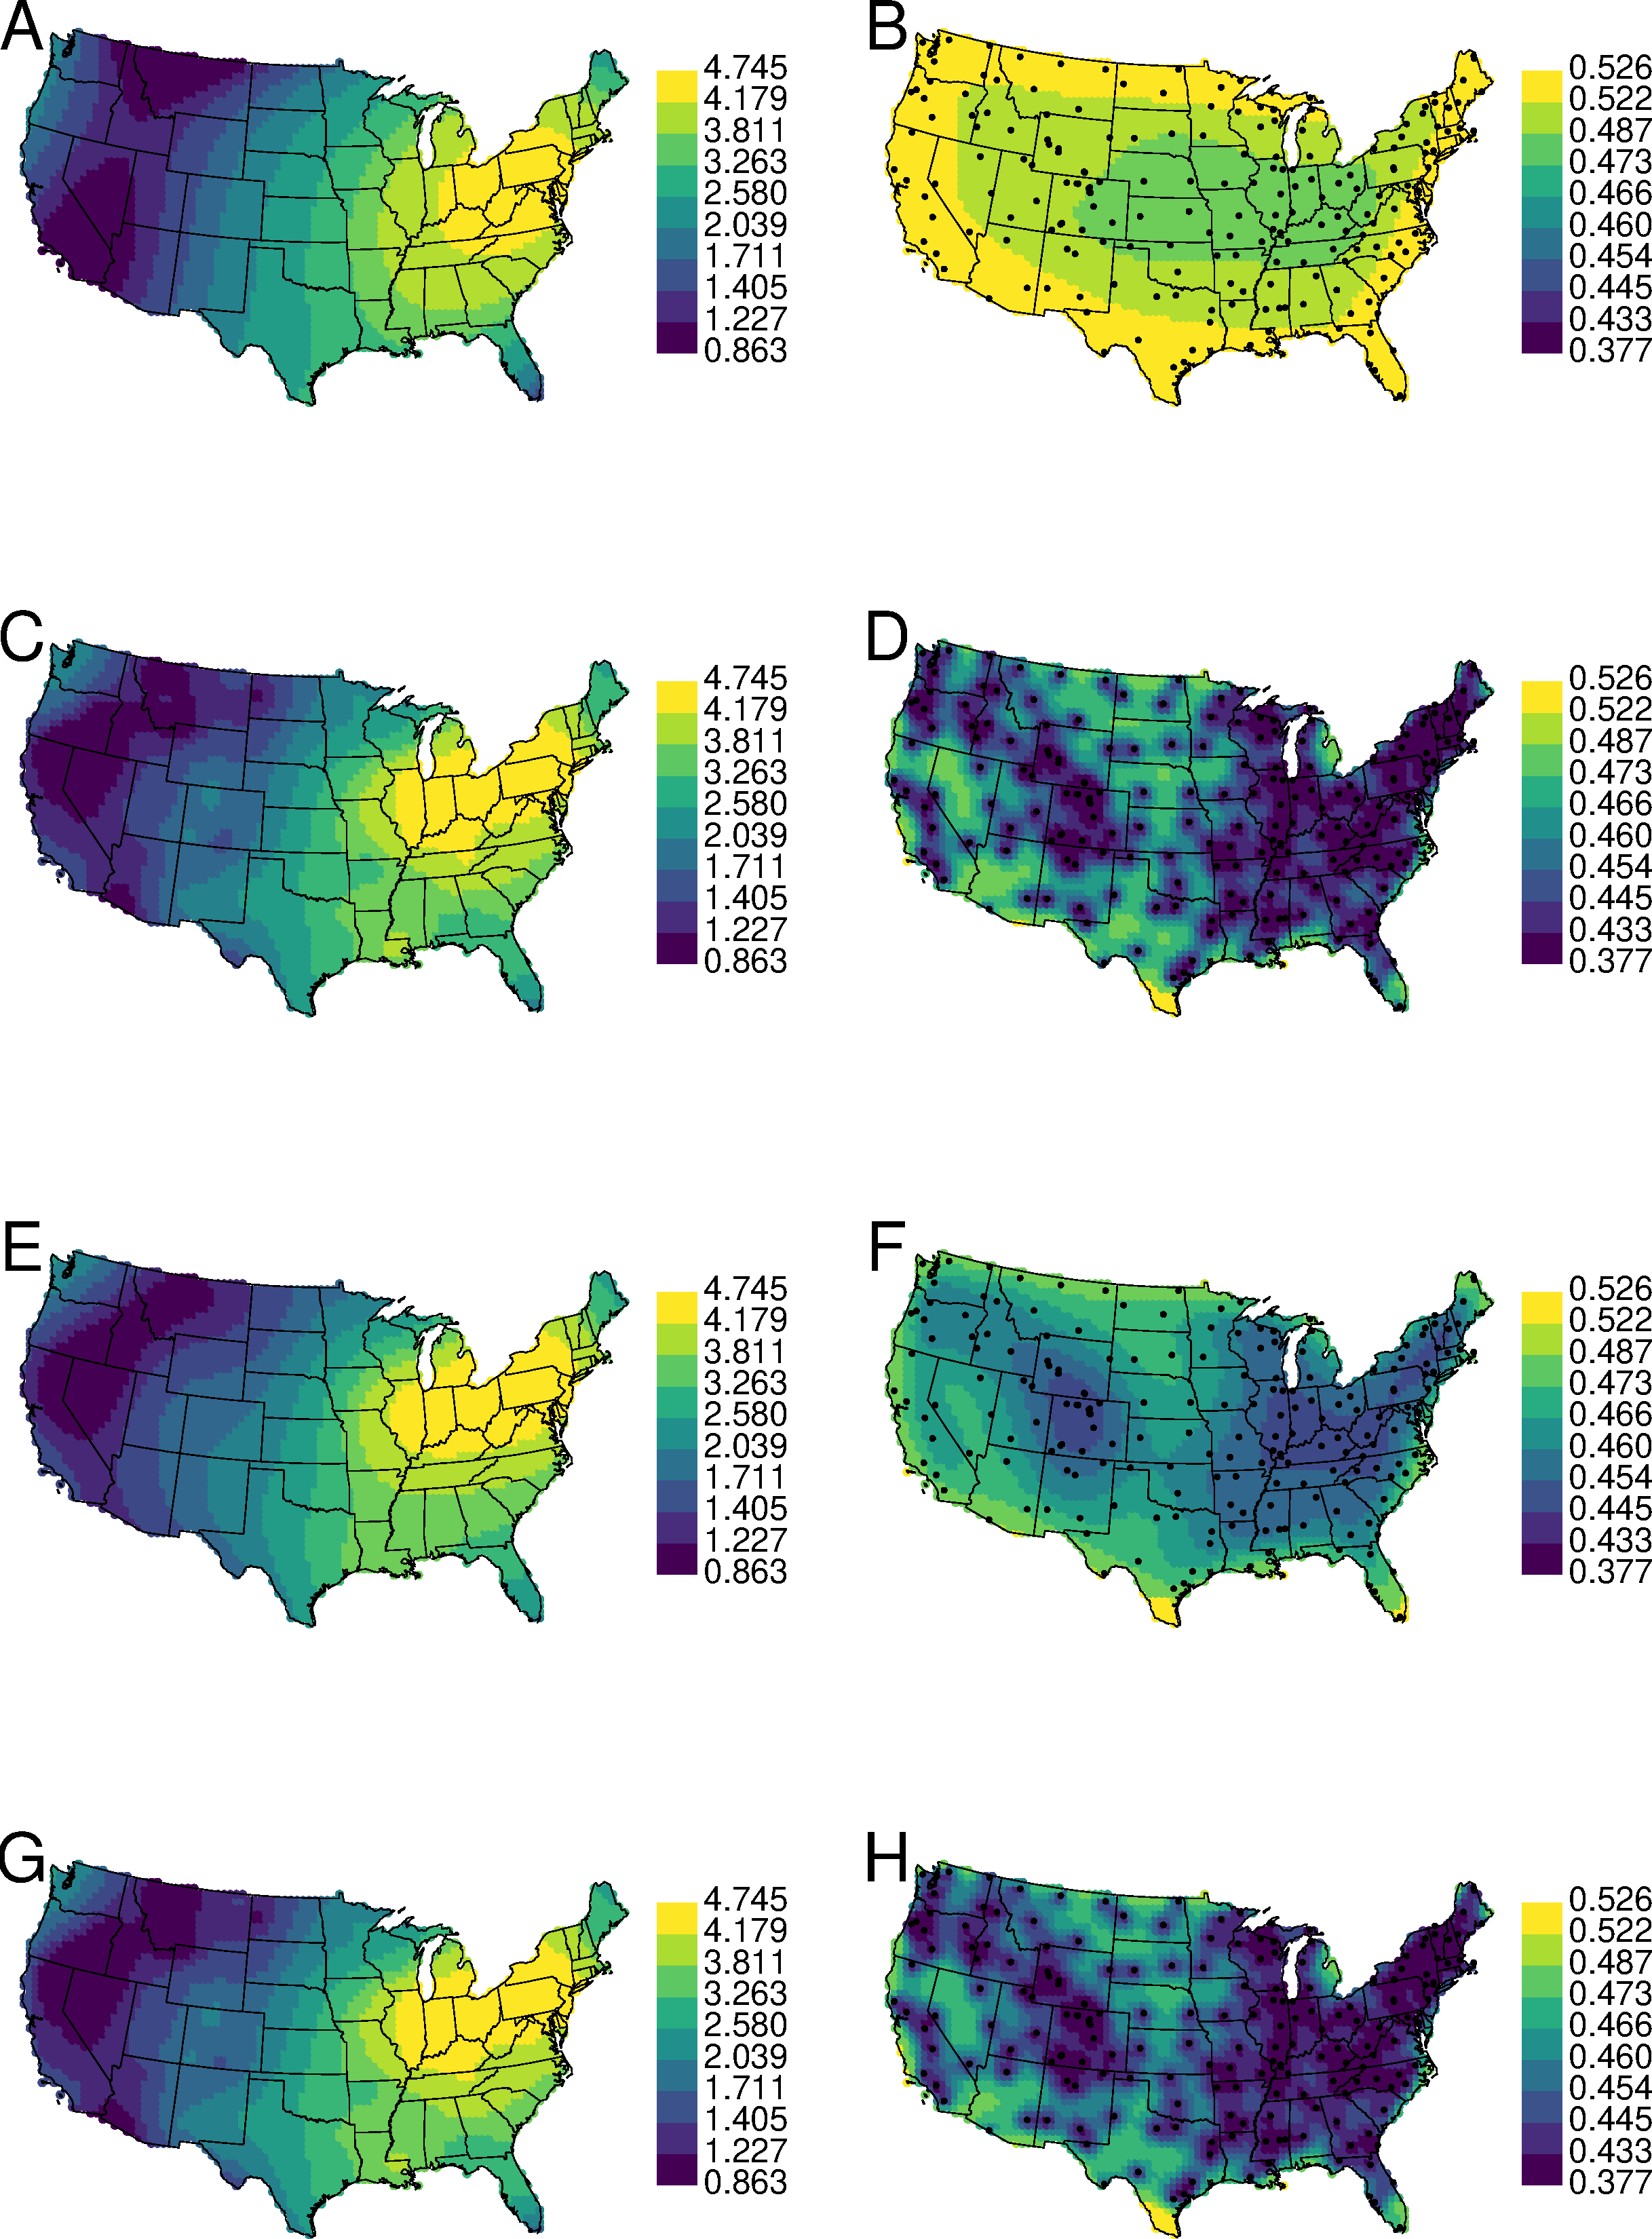
\includegraphics[width=.8\linewidth]{SO4_Prediction_Maps}
  \end{center}
  \caption{Prediction maps (left column) and prediction standard errors (right column) for a variety of models. A-B Fourth-order polynomial assuming independent errors, C-D constant mean spherical model, E-F constant mean exponential model, G-H Third-order polynomial spherical model, I-J constant mean Gaussian model. \label{Fig:SO4_predMaps}}
\end{figure}

%%%%%%%%%%%%%%%%%%%%%%%%%%%%%%%%%%%%%%%%%%%%%%%%%%%%%%%%%%%%%%%%%%%%%%%%%%%%%%%%%%
%%%%%%%%%%%%%%%%%%%%%%%%%%%%%%%%%%%%%%%%%%%%%%%%%%%%%%%%%%%%%%%%%%%%%%%%%%%%%%%%%%
%                BIBLIOGRAPHY
%%%%%%%%%%%%%%%%%%%%%%%%%%%%%%%%%%%%%%%%%%%%%%%%%%%%%%%%%%%%%%%%%%%%%%%%%%%%%%%%%%
%%%%%%%%%%%%%%%%%%%%%%%%%%%%%%%%%%%%%%%%%%%%%%%%%%%%%%%%%%%%%%%%%%%%%%%%%%%%%%%%%%

%\bibliographystyle{consbiol}
\bibliographystyle{/mnt/ExtraDrive1/Work/shTex/asa}
\bibliography{DaleChap883.bib}
%\bibliographystyle{/home/jay/Data/shTex/shTex/asa}
%\bibliography{/home/jay/Data/shTex/shTex/StatBibTex.bib}




\end{document}

